\chapter{Background}\label{c:background}
This section will give a concise background of the mathematical
concepts that will be useful in the sequel, as well as a review of the
literature that this work builds on. It is assumed that the reader is
familiar with multivariable calculus, linear algebra, and the analysis
of algorithms. Section \S\ref{s:notation} gives an overview of the
notational conventions used throughout the remainder of the thesis,
and the remaining sections briefly cover the main results leading up
to my research.

\section*{Notation}\label{s:notation}
% \begin{tabular}[h]{l p{0.8\linewidth}}
{%
\rowcolors{2}{Thistle!10}{white}
\begin{longtable}[h]{|r p{0.8\linewidth}|}
  \hline
  \rowcolor{white}
  \textbf{Symbol} & \textbf{Meaning}\\
  \hline
  $\mathbf{R}$ & The set of real numbers\\
  $\mathbf{R}_+$ & The set of nonnegative real numbers\\
  $\mathbf{N}$ & The set of natural numbers, $\{1, 2,\dots\}$\\
  $\mathbf{N}_0$ & The set of natural numbers including zero, $\mathbf{N}\cup\{0\}$\\
  $2^X$ & The powerset (set of all subsets) of a set $X$\\
  $\mathsf{Set}$ & The category with sets as objects and functions as morphisms\\
  $[N]$ & When $N$ is an integer, $[N]\triangleq\{1,\dots,N\}$.\\
  $\mathscr{B}(\mathcal{A})$ & The Borel $\sigma$-algebra of the
                               topological space $\mathcal{A}$.\\
  $\range(f)$ & The range of a function $f$\\
  $\Expect{f(X)}$ & The expected value of $f(X)$, where $X$ is a
                    random variable\\
  $\ConditionExpect{f(X)}{Y}$ & The conditional expectation of $f(X)$
                                given the value of a random variable $Y$\\
  $X \eqlaw Y$ & Equality in law: the random variables $X,Y$ are
                 distributed identically\\
  $\mathcal{H}(p)$ & The (differential) entropy of a probability
                     distribution $p$\\
  $\mathcal{H}(p, q)$ & The (differential) cross-entropy between
                        probability distributions $p$ and $q$, defined
                        as $\mathcal{H}(p, q) = -\mathbf{E}_{p}[\log q]$\\
  $\uniform{X}$ & The uniform distribution over a bounded
  set $X$\\
  $C(A; B)$ & The set of continuous functions $f:A\to B$, endowed
           with the supremum norm\\
  $C(A)$ & Equivalent to $C(A;B)$ when the output space $B$ is unambiguous\\
  $C^k(A; B)$ & The subset of $C(A;B)$ with functions having continuous
             $k$th derivatives, for $k\in\mathbf{N}$\\
  $C^\infty(A;B)$ & The subset of continuously differentiable functions
                  in $C(A;B)$\\
  $C_c^k(A;B)$ & The subset of $C^k(A;B)$ containing functions that are
               supported on a precompact set, $k\in\mathbf{N}\cup\{\infty\}$\\
  $C_0^k(A;B)$ & The set of functions $f$ in $C_c(A;B)$ that are $0$ on
  the boundary of the support of $f$ (Dirichlet boundary conditions)\\
  $\mathsf{AC}(A)$ & The set of absolutely continuous functions over a
                     set $A$\\
  $\probset{\mathcal{X}}$ & The set of probability measures over a
  measurable space $\mathcal{X}$\\
  $\wassersteinspace[p]{\mathcal{X}}$ & The set of probability
  measures over a set $\mathcal{X}$ endowed with the $p$-Wasserstein metric\\
  $a\land b$ & The minimum of $a$ and $b$\\
  $a\lor b$ & The maximum of $a$ and $b$\\
  $\langle f, g\rangle$ & The inner product between elements
                          $f,g$ of an arbitrary inner product space\\
  $\langle f, g\rangle_{\mathcal{S}}$ & The inner product between vectors $f, g$
                              in an inner product space
                                        $\mathcal{S}$\\
  $\otimes$ & Pointwise (tensor) product: $f\otimes g = x\mapsto f(x)g(x)$\\
  $\indicator{\mathsf{predicate}}$ & The function that takes the value
                                     $1$ when $\mathsf{predicate}$ is
                                     true, and $0$ otherwise\\
  $\characteristic{A}$ & The characteristic function of a measurable
                         set $A$: $\chi_A(x) = \indicator{x\in A}$\\
  $\dirac{z}$ & The Dirac delta distribution\footnote{Note that
                ``distribution'' in this context refers to a
                generalized function, and not a probability
                distribution.}. This is defined such that for any
                function $f$, $\int \dirac{z}(x)f(x)dx = f(z)$.\\
  $\identity$ & The identity function, $\identity(x) = x$\\
  $\trace$ & The trace operator\\
  $\jacobian_{\mathbf{x}}$ & The Jacobian operator for vector-valued functions
  with respect to variable(s) $\mathbf{x}$\\
  $\hessian{\mathbf{x}}$ & The Hessian operator with respect to
                           variable(s) $\mathbf{x}$\\
  $\firstvariation{F}{u}$ & The first variation of a functional $F$
                            with respect to its parameter $u$\\
  $\mathscr{D}(\mathscr{L})$ & The domain of an operator $\mathscr{L}$\\
  $\bot(\cdot)$ & The ``stop gradient operator''. It satisfies
                  $\bot(f)(x)=f(x)$, but $\nabla\bot(f)(x)\equiv 0$\\
  $\proj{k}$ & The projection map to dimension $k$; If $x=(x_1,\dots,
               x_k,\dots x_n)$, then $\proj{k}x=x_k$.\\\hline
\end{longtable}%
}

\section{Reinforcement Learning}
The goal of Reinforcement Learning (RL) is to study how an
\emph{agent} can develop a behavioral policy that is expected to
successfully perform an abstract task, where success is measured by
the \emph{reward} it receives by interacting with the environment. As
an example, we can think of the agent as a humanoid robot that is
rewarded for each second it is balancing on one leg, and penalized
(say, by receiving a negative reward) for falling down. A robot that
receives a high reward in this example will have demonstrated an
ability to balance itself on one foot.

Abstractly, in RL, an agent repeatedly undergoes the following cycle,

\begin{enumerate}
\item The agent observes the present state from the environment;
\item Based on the present state, the agent performs an action of its choice;
\item The agent subsequently transitions to a new state and receives a reward.
\end{enumerate}

The goal of the agent is to maximize the total reward that it
accumulates. Such a setting is formally
described by a \emph{Markov Decision Process}.

\begin{definition}[Markov Decision Process, \citep{puterman2014markov}]
  A \emph{Markov Decision Process} (MDP) is a 5-tuple $(\mathcal{X},
  \mathcal{A}, \mathcal{R}, P, \gamma)$, where
  \begin{enumerate}
  \item $\mathcal{X}$ is a set, called the \emph{state space}, whose
    elements are referred to as \emph{states};
  \item $\mathcal{A}$ is a set, called the \emph{action space}, whose
    elements are referred to as \emph{actions};
  \item $r: \mathcal{X}\to\mathbf{R}$ is
    the \emph{reward function};
  \item $P: \mathcal{X}\times\mathcal{A}\to\mathscr{P}(\mathcal{X})$
    is called the \emph{Markov kernel}, where $P(x'\mid x, a)$ denotes
    the probability of the agent transitioning from state
    $x\in\mathcal{X}$ to state $x'\in\mathcal{X}$ upon performing
    action $a\in\mathcal{X}$;
  \item $\gamma\in(0,1)$ is the \emph{discount factor}, which serves
    the purpose of discounting the value of future rewards.
  \end{enumerate}
\end{definition}

We note that it is common in discrete-time RL to model ``stochastic reward
functions", in which case the reward function $r$ is replaced with an
``augmented" Markov kernel $P^\dagger(x', r\mid x, a)$, which models the
probability density of the next state and reward given the current state and
action. Furthermore, occasionally the return is modeled as a function of both
the current state and action -- note however that the same effect can be
simulated roughly by augmenting each state with the last executed action.
In this thesis, we will only consider deterministic reward functions over the
state space.

It will often be convenient to refer to the probability measure
$P^\pi\in\probset{X\times X}$, given by

\begin{equation}
  \label{eq:p-pi}
  P^\pi(x'\mid x) = \int_{\mathcal{A}}P(x'\mid x, a)\pi(da\mid x)
\end{equation}

where $\pi:\mathcal{X}\to\probset{\mathcal{A}}$ is a \emph{policy}
that samples actions from a state-conditioned distribution.

An important remark about MDPs is that they satisfy the \emph{Markov
  property}, that is, rewards and state transitions are statistically
independent from all states and actions from the past, and depend only
on the present state and action.

Despite the simplicity of the MDP model, the space of problems that
can be formulated as MDPs is enormous \citep{barto1981associative}. In fact, it
has been hypothesized by leading researchers that RL agents can achieve
\emph{artificial general intelligence} \citep{SILVER2021103535}, implying that
they can learn anything that a human can. While RL cannot (yet) achieve
human-level intelligence, RL has successfully achieved superhuman performance in
complex board games like backgammon \citep{tesauro1994td}, chess, Shogi and Go
\citep{silver2018general}, superhuman performance in an entire suite of Atari
video games \citep{mnih2015human, hessel2018rainbow, badia2020agent57}, and
impressive robot control \citep{lin1993scaling, smart2002effective,
peters2003reinforcement, lillicrap2015continuous, higuera2018synthesizing,
bellemare2020autonomous}, among many other accomplishments. 

\subsection{Value-Based Reinforcement Learning}
A common paradigm in RL, known as \emph{value-based} RL, is based on
the concept of learning to associate a notion of ``value'' to each
state, and extracting a behavioral policy that should be likely to
bring the agent to states with high value. The notion of value in RL is
the expected value of the discounted return earned by the agent when
following a given policy. Let $(X_i)_{i=0}^\infty$ denote the sequence of
states visited by an agent in an MDP
$(\mathcal{X},\mathcal{A},r,P,\gamma)$ starting at state
$X_0=x$ -- that is, $X_{k+1}\sim P^\pi(\cdot\mid x)$. Given a measure space $(\mathbf{R}_+,\Sigma,
\mu)$, the discounted return from state $x$ observed by this
trajectory, $G^\pi_\mu(x)$, is given by

\begin{equation}
  \label{eq:return:abstract}
  G^\pi_{\mu}(x) = \Conditional{\int_{0}^\infty\gamma^tr(X_t)d\mu(t)}{X_0 = x}
  % G(x) = \sum_{i=0}^{\infty}\gamma^i\mathcal{R}(X_i)\mid X_0 = x
\end{equation}

In discrete time, $\mu$ is generally chosen to be the \emph{counting
  measure} $\#(A) = |A|, A\in\Sigma$, in which case we have

\begin{equation}
  \label{eq:bg:rl:value-based:return}
  G^\pi_{\#}(x) = \Conditional{\sum_{i=0}^\infty\gamma^ir(X_i)}{X_0 = x}
\end{equation}

When $\mu$ is the counting measure or the Lebesgue measure, we write
$G^\pi_\mu\triangleq G^\pi$, and the context of the problem should immediately
resolve the ambiguity. For the remainder of this chapter, we'll
consider only the discrete-time setting ($\mu=\#$) for a simpler
illustration of the core concepts of RL.

The \emph{value function} $V^\pi:\mathcal{X}\to\mathbf{R}$ for an
agent following policy $\pi:
\mathcal{X}\to\mathscr{P}(\mathcal{A})$\footnote{The policy should be
  interpreted as a conditional probability over actions, e.g. $\pi(a\mid x)
  = \Pr(A_i=a\mid X_i=x)$ for finite state and action spaces.} is
defined as the mapping from states to the expected discounted return:

\begin{equation}
  \label{eq:bg:rl:value-based:value-fn}
  V^\pi(x) = \Expectation{X_i\sim P,
    \pi}{\Conditional{\int_0^\infty\gamma^tr(X_t)d\mu(t)}{X_0 =
      x}} = \ConditionalExpectation{X_{i+1}\sim P^\pi(\cdot\mid
    X_i)}{G^\pi(X_0)}{X_0 = x}
\end{equation}

An observation to note is that (\ref{eq:bg:rl:value-based:value-fn}) can be
written recursively, like so:

\begin{equation}
  \label{eq:bg:rl:value-based:bellman}
  \begin{aligned}
    V^\pi(x) &= \ConditionalExpectation{X_i\sim
      P^\pi}{\int_0^t\gamma^sr(X_s) +
      \gamma^t\int_{0}^\infty\gamma^{s}r(X_{s+t})d\mu(s)}{X_0 = x}\\
    &= \ConditionalExpectation{X_s\sim
      P^\pi}{\int\gamma^sr(X_s)d\mu(s) + \gamma^tV^\pi(X_t)}{X_0 = x}
\end{aligned}
\end{equation}

In the discrete-time setting we have $\mu=\#$ as discussed above, so we can equivalently write

\begin{align*}
  V^\pi(x) = r(x) + \gamma\ConditionalExpectation{X'\sim P^\pi}{V^\pi(X')}{X_0 = x}
\end{align*}

The recursive formulation (\ref{eq:bg:rl:value-based:bellman})
is referred to as \emph{the Bellman equation}
\citep{bellman1954theory}. When the state space is finite, in discrete
time this can simply be expressed as

\begin{equation}
  \label{eq:bg:rl:value-based:bellman:linear}
  \pmb{V}^\pi = \pmb{\mathcal{R}} + \gamma\pmb{P}^\pi\pmb{V}^\pi
\end{equation}

where $\mathcal{X} = \{x_i : i = 1,\dots,|\mathcal{X}|\}$,
$\pmb{V}^\pi\in\mathbf{R}^{|\mathcal{X}|}$ given by $\pmb{V}^\pi_i =
V^\pi(x_i)$, $\pmb{\mathcal{R}}\in\mathbf{R}^{|\mathcal{X}|}$
satisfies $\pmb{\mathcal{R}}_i = r(x_i)$, and
$\pmb{P}^\pi\in\mathbf{R}^{|\mathcal{X}|\times|\mathcal{X}|}$
satisfies $\pmb{P}^\pi_{ij} = P^\pi(x_j\mid x_i)$. It is clear that
(\ref{eq:bg:rl:value-based:bellman:linear}) is linear in the value
function, and given that $\pmb{P}^\pi$ is a stochastic matrix by
construction and $|\gamma|<1$ by definition, we can compute the value
function in closed form:

\begin{equation}
  \label{eq:bg:rl:value-based:bellman:linear:solution}
  \pmb{V}^\pi = \left(I - \gamma\pmb{P}^\pi\right)^{-1}\pmb{\mathcal{R}}
\end{equation}

Note that the inverse $(I - \gamma\pmb{P}^\pi)$ exists since $\pmb{P}^\pi$ is a
stochastic matrix and $\gamma\in(0,1)$ \citep{puterman2014markov}. Of course, it
should be noted that matrix inversion is an expensive
operation, rendering the computation of
(\ref{eq:bg:rl:value-based:bellman:linear:solution}) intractable when
the state space is large.\footnote{Note that we're often interested in
  \emph{continuous} state spaces, which have \emph{uncountable}
  cardinality!} The process of simply determining the
value function corresponding to a fixed policy is a computational
challenge at the core of value-based RL.

Even if we could compute the value function for a fixed policy, in RL
the goal is to find an \emph{optimal} policy. In value-based RL,
policies are compared according to their corresponding value functions
at each state. It is well-known that the existence of an
\emph{optimal} policy according to this criterion is guaranteed
\citep{puterman2014markov} in the discounted infinite horizon
setting\footnote{This refers to the model where agent interacts with
  the environment indefinitely.}
and a policy $\pi^\star$ is optimal if

\begin{equation*}
  \forall\pi\forall x\in\mathcal{X}:V^{\pi^\star}(x)\geq V^\pi(x)
\end{equation*}

Armed with just the knowledge of the value function, determining a
good policy is non-trivial (especially if the reward function and the
transition probabilities are not given). It is convenient to consider
a slightly different mechanism for computing the value function, which
makes use of another mapping known as the \emph{action-value
  function}. For a given policy $\pi$, the action-value function
(referred to as the $Q$-function)
$Q^\pi: \mathcal{X}\times\mathcal{A}\to\mathbf{R}$ is defined as

\begin{equation}
  \label{eq:bg:rl:value-based:q-fn}
  Q^\pi(x, a) = \Expectation{X_i,A_i\sim P,
    \pi}{\Conditional{\sum_{i=0}^\infty\gamma^ir(X_i)}{X_0 =
      x, A_0 = a}} = r(x) + \Expectation{X'\sim P(\cdot\mid
    x, a)}{V^\pi(X')}
\end{equation}

Naturally, one can construct the value function from the action-value
function,

\begin{equation}
  \label{eq:bg:rl:value-based:v-from-q}
  V^\pi(x) = \int_{\mathcal{A}}Q^\pi(x, a)\pi(da\mid x)
\end{equation}

Bellman's principle of optimality, which states that optimal policies
are Markovian \citep{bellman1957markovian}, allows us to characterize
the optimal $Q$-function $Q^{\star}$ via the recurrence

\begin{equation}
  \label{eq:bg:rl:value-based:bellman:optimality}
  Q^\star(x, a) = r(x) + \Expectation{X'\sim P(\cdot\mid x,
    a)}{\max_{a'\in\mathcal{A}}Q^\star(X', a')}
\end{equation}

Given the optimal action-value function and a measure space
$(\mathcal{A},\Sigma_A,\nu)$, it is easy to extract an optimal policy:

\begin{equation}
  \label{eq:bg:rl:value-based:optimal-policy}
  \pi^\star(a\mid x) =
  \frac{d}{d\nu}\characteristic{\arg\max_{a'\in\mathcal{A}}Q^\star(x, a')}
\end{equation}

where $\chi_M$ is the characteristic function of a measurable set $M$,
$\frac{d}{d\nu}$ denotes the Radon-Nikodym derivative operator
with respect to the reference measure $\nu$. In this thesis, we will mainly be
considering MDPs with finite action spaces, so we'll have $\nu=\#$ and an
optimal policy is then given by

\begin{align*}
  \pi^\star(a\mid x) &=
  \frac{1}{|Q^\star(x)|}\indicator{a\in\arg\max_{a'\in\mathcal{A}}Q^\star(x, a')}\\
  |Q^\star(x)| &\triangleq \left\lvert\arg\max_{a'\in\mathcal{A}}Q^\star(x,
    a')\right\rvert
\end{align*}
\subsection{Methods for Estimating the Value Function}
By our discussion in the previous section, we see that the
optimal control problem is easily solved given the knowledge of
the optimal (action-) value function. Unfortunately, usually the
optimal value function is unknown, and determining the optimal value
function can be very challenging. As previously discussed, this can be
accomplished by computing a matrix inversion
(\ref{eq:bg:rl:value-based:bellman:linear:solution}), however there
are several reasons why this is usually not acceptable:

\begin{enumerate}
\item Matrix inversion has cubic time complexity, which is too
  expensive for large or continuous state spaces;
\item This method assumes the agent has knowledge of the precise
  state transition model and the reward function, which is usually not
  assumed to be the case.
\end{enumerate}

Next we will look at some alternative methods for estimating the value
function, each of which circumvent the expensive matrix inversion.

\subsubsection{Policy and Value Iteration}
When the state and action spaces are finite and the transition
probabilities and reward function are known, the optimal value function and an
optimal policy can be approximated efficiently. The \emph{value iteration}
algorithm proposed by \citet{bellman1954theory} uses dynamic programming
\citep{bellman1954theory} to estimate the optimal value function, and extracts an
optimal policy from the estimated optimal value function. More explicitly, if
$\pmb{V}^k\in\mathbf{R}^{|\mathcal{X}|}$ represents the estimate of the optimal value
function after $k$ iterations, we compute $\pmb{V}^{k+1}$ by an application of
the \emph{Bellman optimality operator},

\begin{align*}
  \pmb{V}^{k+1}_x &\leftarrow \pmb{R}_x +
  \gamma\max_{a\in\mathcal{A}}\langle \pmb{P}_{x,a},
  \pmb{V}^k_x\rangle\qquad\forall x\in\mathcal{X}
\end{align*}

where $\pmb{R}\in\mathbf{R}^{|\mathcal{X}|}$ is the vector of rewards at each
state and
$\pmb{P}\in\mathbf{R}^{|\mathcal{X}|\times|\mathcal{X}|\times|\mathcal{A}|}$ is
the matrix of transition probabilities, where $(\pmb{P}_{x,a})_{x'} = P(x'\mid
x, a)$. Upon convergence of the value function, the optimal policy is simply
computed by deterministically mapping each state to the action yielding the
greatest value according to the value function estimate.
It can be shown by a method similar to that shown in
\S\ref{s:background:rl:contraction} that $\pmb{V}^k$ does indeed converge in
$\ell^\infty(\mathbf{R})$ to the optimal value as $k\to\infty$, and for any
given error tolerance the number of iterates required grows logarithmically.
Each iteration can be computed in $O(|\mathcal{X}|^2|\mathcal{A}|)$ time, making
value iteration a substantially more efficient alternative to the matrix
inversion method as the state and action spaces grow.

Another simple method to learn
the action-value function in the discrete state and action space setting is by
\emph{policy iteration} \citep{howard1960dynamic}. Unlike value iteration,
this method iteratively optimizes the estimate of the optimal policy until
convergence while maintaining an estimate of the optimal value function. It
begins with a random guess of both the policy and the value function and
oscillates between update stages known as \emph{policy evaluation} and
\emph{policy improvement}. In the policy evaluation stage, the value function is
updated while fixing the current estimate of the optimal policy, and in the
policy improvement stage the estimate of the optimal policy is updated while
fixing the estimate of the optimal value function. This scheme is conveyed by

\begin{align}
  \pmb{V}^{k+1}_x &\leftarrow \pmb{R}_x + \langle\pmb{P}_{x, \pmb{\pi}^k_x},
  \pmb{V}_x^k\rangle && \forall x\in\mathcal{X}\quad\text{(Policy Evaluation)}\label{eq:policy-evaluation}\\
  \pmb{\pi}^{k+1}_{x} &\leftarrow \arg\max_{a\in\mathcal{A}}\left(\pmb{R}_x +
    \gamma\langle\pmb{P}_{x,a},
    \pmb{V}^{k+1}_x\rangle\right) && \forall x\in\mathcal{X}\quad\text{(Policy
  Improvement)}\label{eq:policy-improvement}
\end{align}

At each iteration, for each state, we compute a value function update requiring
$O(|\mathcal{X}|^2)$ (assuming the mapping $x:\mapsto\pmb{\pi}^k_x$ is a
constant-time operation), plus a policy
update requiring $O(|\mathcal{X}|^2|\mathcal{A}|)$ time, for a total cost of
$O(|\mathcal{X}|^2(1 + |\mathcal{A}|))$ per iteration. It is known that the
policy iterates of this scheme will converge \citep{puterman1979convergence}.
Usually, the
state space is much larger than the action space, so iterations of the
algorithm are considerably less costly than matrix inversion.

\subsubsection{Monte Carlo}
When the transition probabilities and the reward function are not
known, not all hope is lost. Given a generative model of the
environment, we can perform policy evaluation by sampling returns from
the generative model and estimating the expected discounted return
using an unbiased statistical estimator, such as the sample
mean. Suppose the agent starts at a random state $X_0$ sampled from a
distribution $P_0$. We sample $N$ trajectories,

\begin{equation*}
  \begin{aligned}
    A_i^{(k)} &\sim\pi(\cdot\mid X_i^{(k)})\\
    R_i^{(k)}&= \mathcal{R}(X_i^{(k)})\\
    S_{i+1}^{(k)} &\sim P(\cdot\mid X_i^{(k)}, A_i^{(k)})\\
    G_i^{(k)} &= \sum_{j=i}^\infty\gamma^{j-i}R_i^{(k)}\\
  \end{aligned}
\end{equation*}

for $k\in\{1,\dots,N\}$. We then estimate

\begin{equation*}
  V^\pi(X_0) = \frac{1}{N}\sum_{k=1}^NG_0^{(k)}
\end{equation*}

This technique is an example of Monte Carlo sampling. While each value
estimate is not particularly expensive, Monte Carlo methods are known
to exhibit high variance \citep{sutton2018reinforcement}. Consequently, many
samples from the environment are generally required to attain high-fidelity
value estimates. In particular, in order to estimate the action-value function
to within an pointwise error of at most $\epsilon>0$ with probability $1 -
\delta$ for $\delta\in(0,1)$, we must have

\begin{align*}
  N &\geq
  \frac{c}{(1-\gamma)^3}\frac{|\mathcal{X}||\mathcal{A}|\log(c|\mathcal{X}||\mathcal{A}|/\delta)}{\epsilon^2}
\end{align*}

where $c$ is a universal constant and $N$ is the required number of samples
starting from each state \citep{agarwal2019reinforcement}.

\subsubsection{Temporal Difference Learning}
In order to circumvent the high variance of Monte Carlo methods, when
the transition probabilities are not known an alternative method for
estimating the value function is \emph{temporal difference learning}
\citep{sutton1988learning}. In this setting, we begin with an arbitrary
initialization of the value function $V$ and perform updates after
every state transition. That is, at state $x$ we sample

\begin{equation*}
  \begin{aligned}
    a &\sim \pi(\cdot\mid x)\\
    x'&\sim P(\cdot\mid x, a)\\
    r &= \mathcal{R}(x)\\
  \end{aligned}
\end{equation*}

and then we update $V$ according to

\begin{equation*}
  V(x) = \alpha(r + \gamma V(x')) + (1-\alpha)V(x)
\end{equation*}

for some learning rate $\alpha\in(0,1)$. The trick here is that we use our
current ``guess'' of the value
function as our estimate of the tail of the expected return (we are
correcting our guess against a target generated by our guess). This is
called \emph{bootstrapping}, and estimating the expected
return with bootstrapping incurs a bias. Consequently, in accordance
with the bias-variance tradeoff, the variance of temporal difference
learning algorithms tends to be far lower than in Monte Carlo
algorithms, which theoretically suggests that less samples are needed
for an accurate (biased) estimate of the value function. Moreover, it
is known that this bias diminishes and ultimately vanishes as the agent observes
more and more data from the environment \citep{sutton2018reinforcement}, which further
demonstrates that temporal difference learning is a viable technique.

\subsection{Contraction Arguments}\label{s:background:rl:contraction}
A recurring motif in the reinforcement learning literature is the use
of \emph{contraction arguments} to prove that a sequence of value
function iterates converges to a fixed point. Generally, this involves
defining an operator that is \emph{contractive} on the space of value
functions for instance, and ultimately invoking the \emph{Banach fixed
  point theorem}. A brief example will be given. First, we define what
it means for an operator to be contractive. Refer to Appendix
\ref{app:analysis}, particularly \S\ref{s:metric-space}, for a primer on the
topological concepts used in this section.

\begin{definition}[Contraction mapping]\label{def:contraction}
  Let $\mathcal{T}:X\to X$ be an operator on a
  \hyperref[def:metric-space]{metric space} $(X, d)$. We say that
  $\mathcal{T}$ is a \emph{contraction mapping} ($\mathcal{T}$ is
  \emph{contractive}) if for any pair of points $(x, y)\in X\times X$
  we have

  \begin{align*}
    d(\mathcal{T}x, \mathcal{T}y) &\leq \gamma d(x, y)
  \end{align*}

  where $\gamma\in [0,1)$.
\end{definition}

Now we're ready to state the celebrated fixed point theorem of Banach.

\begin{theorem}[Banach's fixed point
  theorem]\label{thm:banach-fixed-point}
  Let $(X, d)$ be a \hyperref[def:complete]{complete} metric space,
  and let $\mathcal{T}:X\times X$ be contractive. Then the sequence
  $\indexedint{k}{\infty}{x}$ where $x_k = \mathcal{T}^k(x_1)$ converges
  to a fixed point $x\in X$, in the sense that $\mathcal{T}x =
  x$. Moreover, this fixed point is unique.
\end{theorem}

\begin{proof}
  For any $x\in X$, we have

  \begin{align*}
    d(x_n, x_m) &\leq d(x_n, \mathcal{T}^nx) + d(x_m, \mathcal{T}^nx)\\
    &\leq \gamma^nd(x_1, x) + \gamma^nd(x_{m-n}, x)\\
    &\to 0
  \end{align*}

  Therefore $\indexedint{k}{\infty}{x}$ is a Cauchy sequence. Since
  $(X, d)$ is complete, it follows that $\indexedint{k}{\infty}{x}$
  converges to some $x^\star\in X$. Since $[0,\infty)$ is known to be
  complete \citep{kreyszig1978introductory}, the sequence
  $\indexedint{k}{\infty}{d}$ where $d_k = d(x_k, x^\star)$ converges
  to $0$, so we see that $d(\mathcal{T}x^\star, x^\star) = 0$. By the
  \hyperref[def:metric-space]{separation of points property} (definition
  \ref{def:metric-space}), we must have $\mathcal{T}x^\star =
  x^\star$. The uniqueness of the fixed point follows from Lemma
  \ref{lem:metric:convergence}.
\end{proof}

We conclude the section by demonstrating a method for learning the
value function using applications of the Bellman equation.

\begin{theorem}[\citet{sutton2018reinforcement}]
  Consider an MDP $(\mathcal{X}, \mathcal{A}, r, P, \gamma)$ and a
  policy $\pi:\mathcal{X}\to\probset{A}$, where $\gamma<1$ and $r$ is
  bounded.
  Denote by $\mathcal{V}$ the
  set of all value functions $V:\mathcal{X}\to\mathcal{R}$ where
  $\mathcal{R}=[\frac{\min_x r(x)}{1-\gamma}, \frac{\max_x r(x)}{1-\gamma}]$.
  We define the Bellman
  operator $\mathcal{T}^\pi:\mathcal{V}\to\mathcal{V}$ according to

  \begin{align*}
    (\mathcal{T}^\pi V)(x) &=
                             \int_{\mathcal{X}\times\mathcal{A}}\left(r(x)
                             + \gamma V(x')\right)dP(x'\mid x, a)d\pi(a)\\
  \end{align*}

  There exists a fixed point $V^\pi$ for $\mathcal{T}^\pi$, and the
  sequence $\indexedint{k}{\infty}{V}$ converges to $V^\pi$ uniformly.
\end{theorem}
\begin{proof}
  Endow $\mathcal{V}$ with the metric $d$ given by $d(V_1, V_2) =
  \sup_{x\in\mathcal{X}}|V_1(x) - V_2(x)|$.
  We will begin by showing that $\mathcal{T}^\pi$ is contractive. We
  have

  \begin{align*}
    d(\mathcal{T}^\pi V_1, \mathcal{T}^\pi V_2)
    &=
      \sup_{x\in\mathcal{X}}\int_{\mathcal{X}\times\mathcal{A}}\lvert
      r + \gamma V_1(x') - (r(x) + \gamma V_2(x'))\rvert dP(x'\mid x, a)d\pi(a)\\
    &=
      \sup_{x\in\mathcal{X}}\int_{\mathcal{X}\times\mathcal{A}}\gamma\lvert
      V_1(x') - V_2(x')\rvert dP(x'\mid x, a)d\pi(a)\\
    &\leq
      \gamma\sup_{x\in\mathcal{X}}|V_1(x) -
      V_2(x)|\int_{\mathcal{X}\times\mathcal{A}}dP(x'
      \mid x, a)d\pi(a)\\
    &= \gamma\sup_{x\in\mathcal{X}}|V_1(x) - V_2(x)|\\
    &= \gamma d(V_1, V_2)
  \end{align*}

  Since $\gamma\in [0,1)$, $\mathcal{T}^\pi$ is indeed a contraction
  map. Moreover, it is known that the metric space $(\mathcal{V}, d)$ presented
  here is complete when the image of $\mathcal{V}$ is complete, which
  is the case since $\mathcal{R}$ is compact
  \citep{kreyszig1978introductory}. Therefore, by the Banach
  fixed-point theorem, the sequence $\indexedint{k}{\infty}{V}$ where $V_k=(\mathcal{T}^\pi)^kV_1$
  converges to a value function $V^\pi$ which satisfies
  $\mathcal{T}^\pi V^\pi = V^\pi$, and $V^\pi$ is the unique solution
  to the fixed point equation for $\mathcal{T}^\pi$. Moreover, the
  convergence is uniform since we have $|V_n(x) -
  V^\pi(x)|\leq\gamma^nd(V_1, V^\pi)$ independently of the state $x$.
\end{proof}

\subsection{Deep Q Networks}\label{s:dqn}
To conclude this brief overview of reinforcement learning, we'll
discuss a particularly successful algorithm that makes the basis of
many state of the art value-based learning algorithms that are around
today. This algorithm, known as \emph{Deep Q-learning}, was famously
employed by the DQN architecture to train an RL agent to outperform
humans in Atari video games \citep{mnih2015human}.

The idea is founded on the concept of Q-learning, which is an RL
algorithm that was classically studied with MDPs having finite state
and action spaces \citep{watkins1989learning}. Rather than learning
the value function, in Q-learning we learn a related concept called
the \emph{action-value function}
$Q:\mathcal{X}\times\mathcal{A}\to\mathcal{R}$ for an MDP
$(\mathcal{X},\mathcal{A},r,P,\gamma)$ with
$\range(r)\subset\mathcal{R}$. This function is defined as

\begin{equation}
  \label{eq:q-function}
  Q(x, a) = \ConditionExpect{\sum_{k=0}^\infty\gamma^kr(x_k)}{x_0
    = x, a_0 = a} = r(x) + \gamma\Expectation{x'\sim P(\cdot\mid x, a)}{V(x')}
\end{equation}

The Q-learning algorithm learns the action-value function (also known
as the $Q$-function) by approximate dynamic programming by iteratively
applying the \emph{Bellman optimality operator}
$\bellmanoperator[\star]$,

\begin{equation}
  \label{eq:bellman-operator:optimality}
  \bellmanoperator[\star] Q(x, a) = r(x) + \gamma\Expectation{x'\sim
    P(\cdot\mid x, a)}{\max_{a'\in\mathcal{A}}Q(x', a')}
\end{equation}

\citet{denardo1967contraction} shows that $\bellmanoperator[\star]$ is
contractive, and so it has a unique fixed point often called
$Q^\star$. However, in many applications of interest, the transition matrix $P$
is unknown, so \eqref{eq:bellman-operator:optimality} cannot be
computed. Fortunately, iterates of
\eqref{eq:bellman-operator:optimality} estimated by data sampled from
the environment are also shown to converge,
resulting in Algorithm \ref{alg:qlearning}.

\begin{algorithm}[h]
  \begin{algorithmic}
    \caption{Q-Learning}\label{alg:qlearning}
    \Require{$Q^i$, the $Q$-function estimated after the $i$th iteration}
    \Require{$\alpha_i\in\mathbf{R}_+$, the ``learning rate'' or
      exponential smoothing parameter}
    \Require{$(s, a)$, a state-action pair.}
    \State{$Q^{i+1}(x, a)\leftarrow Q^i(x, a)\quad\forall (x, a)$}
    \State{$x', r\sim P(\cdot,\cdot\mid x, a)$}\Comment{Sample next state from
      the environment}
    \State{$a'\sim\uniform{\arg\max_{a'\in\mathcal{A}}Q(x',
          a')}$}\Comment{Pick next best action}
    \State{$Q^{i+1}(x, a)\leftarrow \alpha_i(r + \gamma Q^i(x', a') -
      Q^i(x, a))$}
    \State{\Return{$Q^{i+1}$}}
  \end{algorithmic}
\end{algorithm}

Under certain conditions on the sequence $\indexedint{i}{\infty}{\alpha}$, it
is known that $\indexedint{i}{\infty}{Q}\to Q^\star$
\citep{bertsekas1996neuro} when $\indexedint{i}{\infty}{Q}$ is
constructed by applications of Algorithm \ref{alg:qlearning}.

An important observation is that the updates in Algorithm
\ref{alg:qlearning} are independent of the policy that governs the
behavior of the agent in the environment. Consequently, we can perform
the Q-Learning update with \emph{any} transition $(x, a, x')$ sampled
from $P$. Such algorithms are said to be \emph{off-policy}, and are
beneficial in the sense that we may collect a dataset of transitions
and perform updates using this dataset as many times as we'd like,
which makes better use of the data than simply applying an update
using an observed transition and then forgetting about that transition.

Deep $Q$-learning is a framework for performing $Q$-learning
updates in environments with large (even infinite) state spaces, by means
of approximating $Q$ functions by deep neural networks. The DQN
implementation takes advantage of the off-policy nature of
$Q$-learning, and incorporates some additional techniques to stabilize the
learning process.

Firstly, DQN makes use of \emph{experience replay}
\citep{lin1992self}, which consists of storing observed state
transitions in a buffer and performing $Q$-learning updates on
minibatches sampled from the buffer. As well as improving data
efficiency as discussed above, experience replay is also particularly
helpful when training neural networks with stochastic samples. In
order to learn an expected value from samples (such as the
$Q$-function), convergence guarantees can only be made when the
samples used for training are independent and identically-distributed (i.i.d.)
\citep{friedman2017elements}. This is generally not the case in RL,
because consecutive trajectory samples are highly dependent on each
other. By accruing a buffer of transitions and sampling from the
buffer uniformly when performing neural network updates, transitions
are far less dependent on each other. If we keep the policy fixed,
then in the limit as the buffer contains ininitely-many transitions,
all samples from the buffer are distributed according to the
stationary distribution of the Markov chain induced by the
policy. Therefore, experience replay helps by providing the deep
neural networks with approximately i.i.d. data.

Another improvement included in DQN is the use of a \emph{target
  network}. Since the $Q$-function estimate is constantly evolving over the
course of training, the supervised learning problem of mapping
$Q\mapsto r + \gamma Q$ is non-stationary. This severely hinders our
ability to perform policy evaluation. Another tactic to minimize the
non-stationarity involves additionally maintaining a ``target
$Q$-network'' that is updated at a much slower rate. The target
network is used to compute the regression targets, so it is
approximately fixed from the perspective of the predictive
$Q$-network used for inducing a policy. A sketch of DQN is given in
Algorithm \ref{alg:dqn}.

\begin{algorithm}[h]
  \caption[DQN]{DQN, \citet{mnih2015human}}\label{alg:dqn}
  \begin{algorithmic}
    \Require{$Q^1_\theta,Q^1_\phi$, neural nets parameterized by $\theta^1, \phi^1$}
    \Require{$\indexedint{i}{\infty}{\alpha}$, sequence of learning rates}
    \Require{$\tau\in(0,1)$, exponential smoothing parameter}
    \Require{$\pi$, a policy mapping $Q$-values to a probability
      distribution over actions}
    \State{$B\leftarrow\emptyset$}\Comment{Initialize replay buffer}
    \State{$x_1\sim\rho$}\Comment{Sample start state from environment}
    \For{$k\in\mathbf{N}$}
    \State{$a_k\sim\pi(Q^k_\theta(x,\cdot))$}
    \State{$(x_{k+1}, r_k)\sim P(\cdot,\cdot\mid x_k, a_k)$}
    \State{$B\leftarrow B\cup\{(x_k, a_k, r_k,
      x_{k+1})\}$}\Comment{Add transition sample to replay buffer}
    \State{$\theta^{k+1}\leftarrow\theta^k - \alpha_k\nabla_\theta\left(r_k +
        \gamma\arg\max_{a\in\mathcal{A}}Q^k_\phi(x', a) - Q^k_\theta(x_k, a_k)\right)^2$}
    \State{$\phi^{k+1}\leftarrow \tau\phi^k + (1-\tau)\theta^{k+1}$}
    \If{episode is over}
    \State{$x_{k+1}\sim\rho$}\Comment{Reset the environment}
    \EndIf
    \EndFor
  \end{algorithmic}
\end{algorithm}

\section{Stochastic Processes and Differential Equations}\label{s:stochastic-processes}
The material in this section makes extensive use of terminology and
results from \hyperref[app:measure]{measure theory} and
\hyperref[app:stochastic]{stochastic process theory}. An overview of these concepts is
given in Appendices \ref{app:measure} and \ref{app:stochastic}.

Stochastic processes are simply trajectories of random variables
through time. They will be essential in several developments later in
the thesis, and will form the basis for the analysis of the return
distributions.

In order to formalize this concept, we have to introduce the notion of
a \emph{filtration}. A filtration provides us with a mechanism of
``evolving a \hyperref[def:probability-space]{probability space} over
time'', so that the \hyperref[def:measure]{event space}
can in some sense reflect the history of the data previously observed.

\begin{definition}[Filtration,
  \cite{le2016brownian}]\label{def:filtration}
  Let $(\Omega, \mathcal{F}, \Pr)$ be a probability space. A
  \emph{filtration} of $\mathcal{F}$ is a collection
  $(\mathcal{F}_t)_{t\geq 0}$ of
  \hyperref[def:sigma-algebra]{$\sigma$-algebras} where $\mathcal{F}_t\subset\mathcal{F}$
  for each $t$, and $\mathcal{F}_s\subset\mathcal{F}_t$ whenever
  $s<t$. A probability space associated with a filtration is called a
  \emph{filtered probability space}, and is written as the 4-tuple
  $(\Omega, \mathcal{F}, (\mathcal{F}_t)_{t\geq 0}, \Pr)$.
\end{definition}

A Stochastic Differential Equation (SDE) is similar in principle to a
differential equation seen in a standard calculus course, however an
SDE involves stochastic processes. Consider a random process
$\indexedabove{t}{X}$ on a filtered probability space $(\Omega,
\mathcal{F}, \indexedabove{t}{\mathcal{F}}, \mu)$, where
$X_t:\mathcal{F}_t\to\mathcal{X}$ is a 
random variable (it is $\mathcal{F}_t$-measurable) and $\mathcal{X}$
is an arbitrary space that $X_t$ takes values in. For a function
$f:\mathcal{X}\to\mathcal{X}$, we can study the following SDE,

\begin{equation}\label{eq:sde:general}
  Y_t = \int_{0}^tf(Y_s)dX_s,
\end{equation}

where the integral is taken with respect to the stochastic process
$\indexedabove{t}{X}$, and for this thesis it is understood as the
\Ito\ stochastic integral.

\begin{definition}[\Ito\ Integral, \citet{le2016brownian}]
  Consider a filtered probability space $(\Omega, \mathcal{F},
  \indexedabove{t}{\mathcal{F}}, \Pr)$. Let
  $\indexedabove{t}{X}\subset\Omega$ be a
  \hyperref[def:semimartingale]{continuous semimartingale} (Definition
  \ref{def:semimartingale}), and let $f:\Omega\to\Omega$ be defined such that the
  mappings $t\mapsto f(X_t(\omega))$ are continuous for each
  $\omega\in\mathcal{F}_t$. The \emph{\Ito\ integral}
  $\int_0^tf(X_s)dX_s$ is given by

  \begin{align*}
    \int_0^tf(X_s)dX_s = \lim_{n\to\infty}\sum_{i=1}^{p_n - 1}f(X_{t_i^n})(X_{t_{i+1}^n}-X_{t^n_i})
  \end{align*}

  where $\indexedint{i}{p_n-1}{t^n}$ is a partition of $[0,t]$, and
  the sequence of partitions indexed by $n$ have mesh tending to $0$
  as $n\to\infty$.
\end{definition}

Note that $\indexedabove{t}{Y}$ defined in
\eqref{eq:sde:general} is itself a stochastic process. It is common to
express SDEs in a ``differential form''; for instance
\eqref{eq:sde:general} may be written as

\begin{align*}
  dY_t = f(Y_t)dX_t
\end{align*}

although such expressions are merely symbolic.

The remainder of this section will give a general overview of the
concepts from the theory of stochastic processes and differential
equations that are helpful for understanding the remainder of the
thesis. Note that the concepts in this section will not be presented
with full mathematical rigor, as that would likely require a book on
its own \citep{le2016brownian}.

\subsection{Brownian Motion}
Brownian motion is ubiquitous in the study of stochastic
processes. The idea can be motivated as follows.

Let $X_0\triangleq 0\in\mathbf{R}$. Suppose we are modeling the
trajectory of the random process $\indexedabove{t}{X}$, where $X$ is
``continuously perturbed'' by Gaussian noise with mean $0$. What does
it mean for something to be \emph{continuously perturbed} by noise? A
natural way to reason about this is to discretize time, and suppose
that the variable at consecutive timesteps differs by a random
quantity sampled independently from a Gaussian with zero
mean. We want $X_1$ to have variance $1$, and we want this variance to
spread evenly through time in the sense that $X_t$ has variance
$t$. We can begin with a very coarse discretization where the timestep
$\tau$ has duration $1$, which involves sampling
$X_1\sim\gaussian{0}{1}$ and interpolate linearly form $t=0$ to
$t=1$. Then we can study the behavior as $\tau\to 0$. For any
$\tau>0$, we simply sample $X_{t+\tau}\sim X_t +
\gaussian{0}{\tau}$. Alternatively, we can sample 
$(X_{k\tau})_{k\in\mathbf{N}}$ via a
Gaussian process with covariance kernel $K(X_s, X_t) = \min(s, t)$
\citep{williams2006gaussian}. Figure \ref{fig:brownian:viz:1}
illustrates some of these samples for various values of $\tau$.

\begin{figure}[h]
  \centering
  \includegraphics{graphics/brownian.pdf}
  \caption{Discretized Brownian motion trajectories for various
    timesteps $\tau$}
  \label{fig:brownian:viz:1}
\end{figure}

Considering once again the filtered probability space $(\Omega,
\mathcal{F}, \indexedabove{t}{\mathcal{F}}, \mu)$, the criteria for a
Brownian motion $\indexedabove{t}{B}$ can be stated formally as

\begin{enumerate}
\item $B_0=0$, $\mu$-almost surely;
\item For any $0\leq r<s<t$, the random variable $B_t - B_s$ is
  independent from $\mathcal{F}_r$ and is distributed according to
  $\gaussian{0}{t-s}$;
\item The \emph{sample paths} of $\indexedabove{t}{B}$, defined as the
  mappings $t\mapsto B_t(\omega)$ for any fixed
  $\omega\in\mathcal{F}_t$, are continuous.
\end{enumerate}

Proving that such a process exists is not trivial by any
means. Fortunately, Brownian motion \emph{does} exist, and
\citet{le2016brownian} can be consulted for its construction.

\subsection{The Expressivity of \Ito\ Diffusions}\label{s:ito-diffusion}
A recurring motif in this thesis will consist of a special type of
stochastic differential equation known as an \emph{\Ito\
  diffusion}. These are the SDEs of the following form,

\begin{equation}\label{def:ito-diffusion}
  dX_t = a(t, X_t)dt + b(t, X_t)dB_t.
\end{equation}

Since the only source of noise in these types of processes is
Gaussian, it may appear at first glance that the class of solutions to
\Ito\ Diffusion SDEs is fairly limited.
However, it turns out that processes of this form
converge to a very rich class of stationary distributions. This is
nicely stated in the celebrated \emph{Martingale Representation Theorem}.

\begin{theorem}[Martingale Representation Theorem,
  \citet{le2016brownian}]\label{thm:martingale-representation}
  Consider a \hyperref[def:filtration]{filtered probability space}
  $(\Omega, \mathcal{F}, \indexedabove{t}{\mathcal{F}}, \mu)$, where
  $\indexedabove{t}{\mathcal{F}}$ is the completed\footnote{The
    \emph{completion} of a $\sigma$-algebra $\mathcal{F}$ is the
    $\sigma$-algebra generated by $\mathcal{F}$ together with all
    subsets of sets $A\in\mathcal{F}$ that have measure $0$
    \citep{le2016brownian}.} canonical filtration of a Brownian motion
  $\indexedabove{t}{B}$ where $B_0=0$ almost surely. For any random
  variable $Z\in L^2(\Omega, \mathcal{F}_\infty, \mu)$, there exists a
  unique square-integrable \hyperref[def:process:progressive]{progressive
    process} $\indexedabove{t}{h}$ such that

  \begin{equation}
    \label{eq:3}
    Z = \Expect{Z} + \int_0^\infty h_tdB_t.
  \end{equation}
\end{theorem}

Recall the definition of the \hyperref[eq:return:abstract]{random
  return}. Measuring time with respect to the Lebesgue measure, the
return is given by

\begin{align*}
  G^\pi(x) = \int_0^T\gamma^tr(X_t)dt.
\end{align*}

Since $r$ is bounded and $\gamma<1$, $G^\pi(x)$ is obviously square
integrable. Moreover, Brownian motion has infinite variation, and
particles under Brownian motion spread evenly over
$\mathbf{R}$. Therefore, as long as $\law{G^\pi(x)}$ is absolutely
continuous with respect to the Lebesgue measure, we'll have

\begin{align*}
  G^\pi(x)\in L^2(\Omega, \mathcal{F}_\infty, \Pr)
\end{align*}

where $(\Omega, \mathcal{F}, \indexedabove{t}{\mathcal{F}}, \Pr)$ is
the probability space $\mathsf{P}$
\hyperref[def:probability-space]{defined} above. Therefore, \emph{any}
return distribution that is absolutely continuous with respect to the
Lebesgue measure can be expressed as the stationary distribution of an
\Ito\ diffusion.

The most difficult part when dealing with stochastic differential
equations (SDEs) is, unsurprisingly, the stochastic integral. It would
be desirable then if we could express a random variable as the
solution to an SDE of the form

\begin{equation}
  \label{eq:langevin}
  dZ_t = -\nabla \phi(t, Z_t)dt + dB_t
\end{equation}

for some twice differentiable function $\phi$. The SDE
\eqref{eq:langevin} is an example of \emph{Langevin dynamics}, and the
method of representing random variables via Langevin dynamics has
become popular in the machine learning literature in recent years
\citep{welling2011bayesian, wibisono2018sampling, raginsky2017non}. In
the context of reinforcement learning, \citet{Zhang2018PolicyOA}
represents the evolution of a parameterized policy as a set of
particles in parameter space under the influence of Langevin dynamics. Moreover,
\citet{martin2020stochastically} exhibits a similar technique in the
discrete-time value-based setting.

Let $(\Omega, \mathcal{F}, \indexedabove{t}{\mathcal{F}})$ be a
filtered measurable space on which $\indexedabove{t}{B}$ is a Brownian
motion with respect to a probability measure $\mu$. The following
theorem will enable us to transform a Brownian motion to Langevin dynamics.

\begin{theorem}[Girsanov's Theorem, \citep{girsanov1960transforming}]
  Let $(\Omega, \mathcal{F})$ be a measurable space and let
  $\indexedabove{t}{\mathcal{F}}$ be a filtration of
  $\mathcal{F}$. Suppose $\mu,\nu$ are measures on $(\Omega,
  \mathcal{F})$ which are absolutely continuous with respect to one
  another on $\mathcal{F}_\infty$. Let $\indexedabove{t}{D}$ be the
  martingale with c\`adl\`ag\footnote{This refers to functions that
    are \emph{continue \`a droite, limites \`a gauche} -- that is --
    right continuous functions with left limits.} sample paths such
  that for every $t\geq 0$ we have
  \begin{align*}
    D_t = \frac{d\nu}{d\mu\rvert_{\mathcal{F}_t}}
  \end{align*}

  where $\mu\vert_{\mathcal{F}_t}:\mathcal{F}_t\to\mathbf{R}_+$ is the measure
  $\mu$ restricted to the domain $\mathcal{F}_t$.

  Let $\indexedabove{t}{[L,L]}$ denote the
  \hyperref[def:quadratic-variation]{quadratic variation} of
  $\indexedabove{t}{L}$ (shown in Definition \ref{def:quadratic-variation} of
  Appendix \ref{app:stochastic}).
  Assume that $D$ has continuous sample paths, and let $L$ be the
  \hyperref[def:local-martingale]{continuous local martingale} such that

  \begin{align*}
    D_t = \exp\left(L_t - \frac{1}{2}[L,L]_t\right)
  \end{align*}

  Then if $M$ is a continuous local martingale under $\mu$, $\indexedabove{t}{M -
  [M,L]}$ is a continuous local martingale under $\nu$, where
  $\indexedabove{t}{[M,L]}$ is the \hyperref[def:bracket]{bracket} of
  $\indexedabove{t}{M},\indexedabove{t}{L}$ as shown in Definition
  \ref{def:bracket} of Appendix \ref{app:stochastic}.
\end{theorem}

Let $\nu$ be a probability measure on $(\Omega, \mathcal{F})$ that is
absolutely continuous with respect to $\mu$. We'll additionally impose
the constraint that $\nu_1 = \text{Law}(Z_1)$. Girsanov's theorem
tells us that

\begin{equation}\label{eq:langevin:girsanov}
  \frac{d\nu}{d\mu} = \exp\left(-\int_0^1\langle\nabla \phi(B_t,
  t),dB_t\rangle - \frac{1}{2}\int_0^1\|\nabla \phi(B_t, t)\|^2dt\right)
\end{equation}

Let $\mathcal{M}_{Z_1} = \{\nu\in\probset{\Omega} : \nu_1 =
\text{Law}(Z_1)\}$, where $\probset{\Omega}$ is the set of
probability measures on $(\Omega, \mathcal{F})$. Then we'll define our
target measure $\nu^\star$ by

\begin{align*}
  \nu^\star = \arg\min_{\nu\in\mathcal{M}_{Z_1}}\kl{\nu}{\mu}
\end{align*}

The reason for this specification is that the chain rule of the KL
divergence yields

\begin{align*}
  \kl{\nu^\star}{\mu} &=
                        \arg\min_{\nu\in\mathcal{M}_{Z_1}}\left[\kl{\nu_1}{\mu_1}
                        + \int\nu_1(dx)\kl{\nu(\cdot\mid
                        Z_1=x)}{\mu(\cdot\mid Z_1=x)}\right]\\
  &= \kl{\text{Law}(Z_1)}{\mu_1}
\end{align*}

where the final step follows since the only constraint on $\nu$ occurs
at $\nu_1$, so we can minimize the KL divergence by ensuring that
$\mu=\nu$ almost everywhere. But since Brownian motion has independent
increments and $\mu=\nu$ almost everywhere, it follows that

\begin{align*}
  \frac{d\nu}{d\mu} &= \varrho(Z_1)
\end{align*}

for some function $\varrho$. Consequently, we see that
$\frac{d\nu}{d\mu}$ must correspond to the density of $Z_1$.

Proceeding, we'd like to find a way to eliminate the stochastic
integral from \eqref{eq:langevin:girsanov}. Fortunately, we can do so
by exploiting \hyperref[app:ito]{\Ito's lemma}. Let  $U_t = \phi(B_t,
t)$. Then

\begin{align*}
  dU_t &= \partialderiv{\phi}{t}(B_t, t)dt + \frac{1}{2}\Delta\phi(B_t, t) +
         \langle\nabla\phi(B_t, t), dB_t\rangle\\
\end{align*}

Note that the final term above is equivalent to the integrand in
\eqref{eq:langevin:girsanov}. Integrating yields

\begin{align*}
  U_1 &= U_0 + \int_0^1\left[\partialderiv{\phi}{t}(B_t, t) +
        \frac{1}{2}\Delta\phi(B_t, t)\right]dt + 
        \int_0^1\langle\nabla\phi(B_t, t), dB_t\rangle\\
\end{align*}

Upon substitution into \eqref{eq:langevin:girsanov}, we have

\begin{equation}
  \label{eq:langevin:nosde}
  \frac{d\nu}{d\mu} = \exp\left(U_0 - U_1 +
    \int_0^1\left[\partialderiv{\phi}{t}(B_t, t) +
      \frac{1}{2}\Delta\phi(B_t, t) -
      \frac{1}{2}\|\nabla\phi(B_t, t)\|^2\right]dt\right)
\end{equation}

Recall that $\frac{d\nu}{d\mu}$ should be expressed as a function of
$Z_1=B_1$ only. Since $B_0 = 0$ almost surely, it follows that the
integral in \eqref{eq:langevin:nosde} must vanish. This presents us
with the following characterization of the function $\phi$ such that
$\text{Law}(Z_1) = \nu_1$,

\begin{equation}
  \label{eq:langevin:pde}
  \partialderiv{\phi}{t} + \frac{1}{2}\Delta\phi -
  \frac{1}{2}\|\nabla\phi\|^2 = 0
\end{equation}

Letting $h\triangleq e^{-\phi}$, we see that

\begin{align*}
  0 &= -\partialderiv{\log h}{t} - \frac{1}{2}\Delta(\log h) -
  \frac{1}{2}\|\nabla(\log h)\|^2\\
  &= \frac{1}{h}\partialderiv{h}{t} +
    \frac{1}{2}\nabla\cdot\frac{\nabla h}{h} +
    \frac{1}{2}\left\|\frac{1}{h}\nabla h\right\|^2\\
  &= \frac{1}{h}\partialderiv{h}{t} +
    \frac{1}{2}\left[\frac{1}{h}\Delta h - \frac{1}{h^2}\|\nabla
    h\|^2\right] + \frac{1}{2}\left\|\frac{1}{h}\nabla h\right\|^2\\
  &= \partialderiv{h}{t} + \frac{1}{2}\Delta h
\end{align*}

Therefore, $h = e^{-\phi}$ satisfies the \emph{heat equation}
\citep{harrison2013brownian, ullrich2011time}! Explicitly, we want to
solve the following boundary value problem for a function $h:\mathcal{X}\times[0,1]\to\mathbf{R}$,

\begin{equation}
  \label{eq:langevin:bvp}
  \begin{cases}
    \partialderiv{h}{t} + \frac{1}{2}\Delta h = 0 \\
    h(x, 1) = \psi(x)\\
  \end{cases}
\end{equation}

where $\psi$ encodes a terminal condition. The Feynman-Kac formula
\citep{kac1949distributions} (discussed in \S\ref{app:feynman-kac}) famously
shows\footnote{In fact, \eqref{eq:langevin:bvp} is simply a \emph{Kolmogorov
backward equation}, which will be discussed in more detail
\hyperref[thm:kbe]{later in the thesis}.} that \eqref{eq:langevin:bvp} is
satisfied by

\begin{equation}
  \label{eq:langevin:bvp:solution}
  h(x, t) = \ConditionExpect{\psi(B_1)}{B_t = x}
\end{equation}

And equivalently, this provides us with the following characterization
of $\phi$,

\begin{equation}
  \label{eq:langevin:phi}
  \phi(x, t) = -\log\ConditionExpect{\psi(B_1)}{B_t=x}
\end{equation}

When \eqref{eq:langevin:phi} is satisfied, \eqref{eq:langevin:nosde}
becomes

\begin{align*}
  \frac{d\nu}{d\mu} &= \exp(U_0 - U_1)\\
                    &= \exp(\phi(B_0, 0) - \phi(B_1, 1))\\
  &= \exp(\log\psi(B_1))\\
  &= \psi
\end{align*}

This tells us that $\psi\equiv\varrho$, the density of
$B_1=Z_1$. Finally, we see that the stationary solution of the SDE

\begin{equation}
  \label{eq:langevin:solution}
  dZ_t = \nabla\log\ConditionExpect{\varrho(Z_1)}{Z_t}dt + dB_t
\end{equation}

will have density $\varrho$.

\begin{remark}
  Notably, no convexity assumptions are necessary for this
  convergence.
\end{remark}

\begin{remark}
  Unlike sampling algorithms based on Markov Chain Monte Carlo (MCMC)
  such as Metropolis Hastings \citep{hastings1970monte},
  we have a guarantee that at time $t=1$ we'll have \emph{an exact
    sample} from $\varrho$. However, in many cases, computing
  $\nabla\ConditionExpect{\varrho(Z_1)}{Z_t}$ exactly will not be
  tractable, and additionally simulating \eqref{eq:langevin:solution}
  will accrue error due to time discretization.
\end{remark}

In the statistics and machine learning literature, sampling via such
Langevin diffusions is common practice
\citep{roberts2002langevin}. The technique has been used in particular
to extend existing algorithms to a Bayesian treatment. The Stochastic
Gradient Langevin Diffusion (SGLD) framework
\citep{welling2011bayesian}, for example, simulates Langevin
diffusions in parameter space to produce a Bayesian extension of
Stochastic Gradient Descent (SGD), which is used to compute posterior
distributions over large parameterized models.

\section{Continuous-Time Dynamics}
So far, we've discussed algorithms that learn control policies that
evolve in discrete timesteps. While every computer program must evolve
discretely in time, we may be interested (and we will be for the sake
of this thesis) in how reinforcement learning algorithms behave as the
timestep duration tends to $0$. Mathematics become far more technical
in this regime, since the infinitesimal differentials between some
quantities may not be well defined. As we'll see below, even in the
absense of any uncertainty, continuous-time optimal control presents
considerable difficulties.

\subsection{The Deterministic Case}
A well-known result from optimal control theory is that when the
optimal value function is differentiable, it satisfies the following
equation,

\begin{equation}
  \label{eq:dynamic-programming}
  V(x)\log\gamma + \sup_{a\in\mathcal{A}}\left[r(x, a) + \langle\nabla
    V(x), f(x)\rangle\right] = 0
\end{equation}

where $\mathcal{A}$ is the action space,
$r:\mathcal{X}\times\mathcal{A}\to\mathbf{R}$ is the reward function,
$\dot{x}(t) = f(x(t), a(t))$,
and the optimal value function $V(x)$ is defined as

\begin{equation}
  \label{eq:value-function-continuous}
  V(x) = \sup_{a(\cdot)\in
    L^1(\mathbf{R}_+}\int_0^\infty\gamma^tr(x(t), a(t))dt\qquad x(0) = x
\end{equation}

Equation \eqref{eq:dynamic-programming} is known as the
\emph{Hamilton-Jacobi-Bellman} (HJB) equation
\citep{fleming2006controlled}.\footnote{Some texts refer to this
  equation as the \emph{dynamic programming equation}. However,
  ``dynamic programming'' refers to an algorithmic technique for
  solving such equations \citep{bellman1954theory}, so we prefer to
  avoid this nomenclature.} The HJB equation takes
on a similar form to the Bellman equation, but we note one immediate
difference: the Bellman equation expresses $V$ recursively, and the
HJB equation expresses it \emph{differentially}. This is to be expected, however, since the
HJB equation can be interpreted as the limiting equation when
consecutive states are separated by an infinitesimal time in the
Bellman equation. Of course, that only makes sense if we
\textbf{assume that the universe does not stop and wait for us in
  between timesteps of an MDP}.

Rather than a recurrence relation, the HJB equation presents us with a
nonlinear partial differential equation (PDE). PDEs are notoriously difficult to solve, so already
continuous-time RL looks discouraging. However, the challenges do not stop there. Recall that
the optimal value function satisfies \eqref{eq:dynamic-programming}
\emph{if it is differentiable}, but what happens when it is not
differentiable? This may seem like merely a technicality for at least
a couple of reasons:

\begin{enumerate}
\item It may seem like we can just avoid the issue altogether by
  approximating the value function somehow, and possibly weakening the
  notion of solutions to \eqref{eq:dynamic-programming};
\item Perhaps the consequences of assuming the value function is
  differentiable in practice are negligible?
\end{enumerate}

We will proceed by showing that this phenomenon is in fact problematic both in
theory and in practice.

The following is an example due to
\citet{Munos2004ASO}. Consider a continuous-time MDP where
\begin{itemize}
\item The state space $\mathcal{X} = [0,1]$;
\item The action space $\mathcal{A} = \{-1, 1\}$;
\item The dynamics are given by $\dot{x}(t) = a(t)$ where $x(\cdot)$
  is the state signal and $a(\cdot)$ is the control signal;
\item The reward function is $r(x) = \dirac{0}(x) + 2\dirac{1}(x)$;
\item Episodes run until the agent exits the interior of
  $\mathcal{X}$.
\end{itemize}

This problem seems exceptionally simple at first glance. So simple, in
fact, that we can easily plot the optimal value function, as shown in
Figure \ref{fig:munos:value}.

\begin{figure}[h]
  \centering
  \includegraphics{graphics/munos-value.pdf}
  \caption[A non-differentiable value function]{Value function from
    Munos' toy problem, $\gamma=0.3$}\label{fig:munos:value}
\end{figure}

As Figure \ref{fig:munos:value} indicates, the value function for this
problem is not differentiable everywhere. We'll proceed by assessing
our first skepticism: why can't we just approximate the value function
by a differentiable function? As a matter of fact, we \emph{can} do
this, however the approximation is far from trivial. Looking at
\ref{fig:munos:value}, it is reasonable to suggest that we simply
search for $V$ among piecewise differentiable functions, or even
Sobolev spaces. Clearly in this case we'd still find the value
function, as it is piecewise differentiable. However, this absolutely
does not solve the problem, not even for this one example environment:
it is well-known that there are infinitely many functions
differentiable almost everywhere that satisfy
\eqref{eq:dynamic-programming} \citep{fleming2006controlled}!
\citet{Munos2004ASO} demonstrates that solutions to the HJB equation
can be vastly dissimilar to the value function. Consequently,
attempting to search for a solution to the HJB equation among
functions that are differentiable almost everywhere using gradient
based methods is likely to converge to a local optimum, and the local
optimum can be entirely unrepresentative of the true value function.

Fortunately, not all hope is lost. The celebrated work of
\citet{crandall1983viscosity} introduces a weak interpretation of
solutions to the HJB equation, namely \emph{viscosity solutions}, for
which there exists a unique solution among the space of
almost-everywhere-differentiable functions.

\begin{definition}[Viscosity solution,
  \citep{crandall1983viscosity}]\label{def:viscosity}
  Let $\mathcal{O}\subset\mathbf{R}^d$ be an open set. We define
  set-valued functions $E_+, E_-: C(\mathcal{O})\to 2^{\mathcal{O}}$
  according to

  \begin{align*}
    E_+(\psi) &= \left\{y\in\mathcal{O} : y\in\arg\max\psi\land\psi(y)>0\right\}\\
    E_-(\psi) &= \left\{y\in\mathcal{O} : y\in\arg\min\psi\land\psi(y)<0\right\}\\
  \end{align*}

  We consider equations of the form $H(y, V, \nabla V) = 0$ for a
  continuous function
  $H:\mathcal{O}\times\mathbf{R}\times\mathbf{R}^d\to\mathbf{R}$.
  A function $v\in C(\mathcal{O})$ is said to be a \textbf{viscosity
    subsolution} of $H(y, V, \nabla V)=0$ if for every positive
  function $\phi\in C^\infty_c(\mathcal{O})$ and $k\in\mathbf{R}$ we
  have

  \begin{align*}
    E_+(\phi(v - k))\neq\emptyset\implies&\exists y\in E_+(\phi(v -
                                   k)):\\
    &\quad H\left(y, v(y), -\frac{v(y) - k}{\phi(y)}\nabla\phi(y)\right)\leq 0
  \end{align*}

  Similarly, a function $v\in C(\mathcal{O})$ is called a
  \textbf{viscosity supersolution} of $H(y, v, \nabla V)=0$ if for
  every positive $\phi\in C_c^\infty(\mathcal{O})$ and
  $k\in\mathbf{R}$ we have

  \begin{align*}
    E_-(\phi(v - k))\neq\emptyset\implies&\exists y\in E_-(\phi(v -
                                   k)):\\
    &\quad H\left(y, v(y), -\frac{v(y) - k}{\phi(y)}\nabla\phi(y)\right)\geq 0
  \end{align*}

  Finally, a function $v\in C(\mathcal{O})$ is called a
  \textbf{viscosity solution} of $H(y, V, \nabla V)=0$ if for this
  equation it is both a viscosity subsolution and a viscosity supersolution.
\end{definition}

The beauty of viscosity solutions lies in the fact that the optimal
value function is the unique viscosity solution for a given HJB
equation \citep{crandall1983viscosity}. Based on the stability and
regularity properties of viscosity solutions, \citet{munos1997convergent}
presents a convergent reinforcement learning algorithm that employs a
finite-differences scheme to solve the HJB equation.

Now we turn to our second skeptical question: does this even matter in
practice? We can answer this affirmitively by demonstration. We
implement an algorithm like that described in
\citet{munos1997convergent} and compare its performance to
$Q$-learning in this toy example. The results are shown in Figure
\ref{fig:munos:value:comparison}.

\begin{figure}[h]
  \centering
  \newcommand{\munosvaluecomparisonscale}{0.38}
  \begin{minipage}[h]{0.49\linewidth}
    \centering\textsc{Q-Learning}\\
    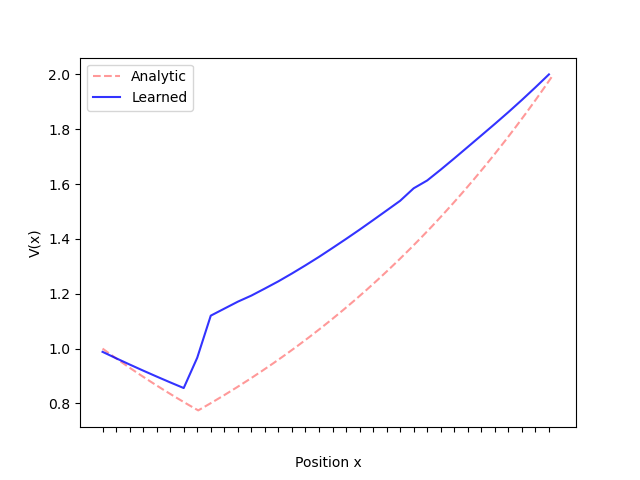
\includegraphics[scale=\munosvaluecomparisonscale]{results/dt-munos-value}
  \end{minipage}%
  \begin{minipage}[h]{0.49\linewidth}
    \centering\textsc{Finite Differences}\\
    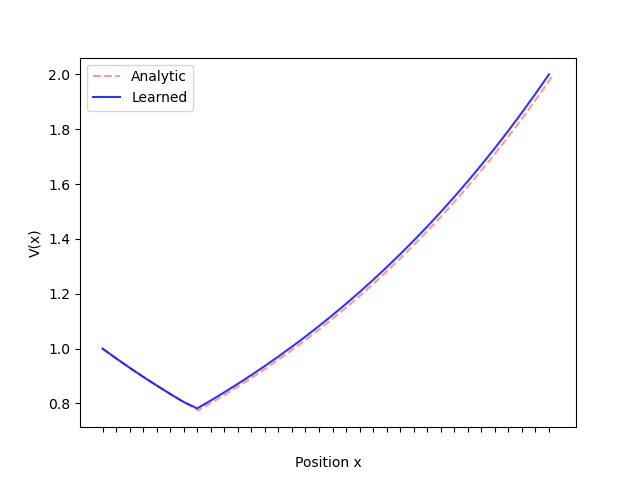
\includegraphics[scale=\munosvaluecomparisonscale]{results/ct-munos-value}
  \end{minipage}
  \caption[Failure of Q-learning in continuous time]{Value functions
    learned by a continuous-time RL algorithm and Q-Learning for
    Munos' toy example}
  \label{fig:munos:value:comparison}
\end{figure}

In our experiments, we use a small timestep duration $\tau=10^{-3}$
and we discretize the state space uniformly into $100$
bins. Hyper-parameter search for the optimal learning rate sequence
was conducted identically for both algorithms. We see that
$Q$-learning converged to a value function with a discontinuity near
the point of non-differentiability of the value function. Consequently
the value function learned by $Q$-learning is only approximately
correct near the boundaries of the state space. On the other hand, the
algorithm with continuous-time corrections learns a continuous value
function that approximates the viscosity solution of
\eqref{eq:dynamic-programming} well on the entire state space.

Beyond this simple environment, \citet{doya2000reinforcement} presents
a number of algorithms that are extensions of existing (discrete-time)
RL algorithms to the continuous time setting, including a method with
differential updates based on the gradient of the value function, and
encorporating $\text{TD}(\lambda)$ updates \citep{sutton1988learning}
to reduce bias. This algorithm was reported to have learned optimal
controllers for complex control tasks faster than discrete-time
counterparts by a substantial amount.

\subsection{Unveiling Problems in Discrete Reinforcement Learning}
Another reason for studying reinforcement learning in the
continuous-time setting is that it forces us to recognize some of the
technical challenges of reinforcement learning that are obscured, but
still present, in the discrete-time MDP model. One such example is 
part of the credit assignment problem, which is the problem of
determining which actions from a given episode in an MDP contributed
most to the return. This problem is certainly addressed in the
reinforcement learning literature \citep{sutton1984temporal,
  arumugam2021information}, however the study of reinforcement
learning in continuous time demonstrates a new challenge.

The work of \citet{baird1993advantage} presents an interesting
challenge for credit assignment when the timestep is small (or
infinitesimal). For systems evolving continuously in time, we expect
different controls to have similar $Q$-values at a given state -- that
is, individual actions should not perturb the overall return too
greatly. In fact, it is shown in \citet{baird1993advantage} and
formally proved in \citet{tallec2019making} that as
the timestep shrinks, the $Q$-function may completely disregard the
action altogether. In that case, $Q$-learning at the very least should
be expected to learn extremely slowly, if at all. In order to correct
this, the \emph{Advantage Updating} algorithm is presented, where
``advantage'' functions are learned as opposed to $Q$-functions, and
the advantage functions $A$ are related to the $Q$-functions via

\begin{equation}
  \label{eq:advantage-updating}
  A(x, a) = \frac{1}{\tau}\left(Q(x, a) - \max_{a'\in\mathcal{A}}Q(x, a')\right)
\end{equation}

where $\tau$ is the duration of the timestep. By effectively scaling
$Q$-functions by $\tau^{-1}$, the advantage functions do not lose
information about actions in the continuous time limit, and
\citet{baird1994reinforcement} reports that advantage learning
converged $10^5$ times faster than $Q$-learning in their
experiments. The work of \citet{bellemare2016increasing} develops
further on this idea by demonstrating a class of ``consistent''
Bellman-like operators, and empirical results in complex experiments
using consistent updates substantially improve over previous similar
RL algorithms.

Another approach to solving the continuous-time credit assignment
problem was recently suggested by \citet{kim2021hamilton}, which
presents the Hamilton-Jacobi Deep Q Network (HJ-DQN). This framework
allows us to perform value-based RL when the action space is
continuous, under the assumption that the control signal is
Lipschitz-continuous in time. This assumption effectively means that
the control is not changing too quickly, so the individual controls
have more influence on the final return. Moreover, by the definition
of Lipschitz-continuity, the time-derivative of the control signal is
bounded by some constant $L$ and we can determine the optimal action
at each timestep (even though there are infinitely many candidates!)
by

\begin{align*}
  \dot{a}(t) &= L\frac{\nabla_aQ(x, a)}{\|\nabla_a Q(x, a)\|}
\end{align*}

Simply put -- we must determine the direction in action space that
maximizes the $Q$-function most quickly by computing the $a$-gradient
of the $Q$ function, and then perturb the control as much as we're
allowed to by the Lipschitz constraint in that direction.

A similar feat can be accomplished if we make an alternative
assumption that the dynamics are \emph{control-affine}, meaning
$\dot{x}(t) = f(x(t)) + \langle g, a(t)\rangle$ for some linear
operator $g$ and arbitrary function $f$. In particular, under this
class of dynamics, value-maximizing actions can be computed in closed
form even when the action space is uncountable
\citep{tassa2007least}. Recently, this idea was applied with great
success in the Continuous Fitted Value Iteration (cFVI) algorithm
\citep{lutter2021value} and in the Robust Fitted Value Iteration
(rFVI) algorithm \citep{lutter2021continuous}. 

The study of \citet{tallec2019making} also discusses what is a
seemingly un-explored parameter of reinforcement learning models: the
length of the timestep. Even when the timesteps are not miniscule, it
is not unreasonable to suspect that RL algorithms might perform
differently due to changes in the timestep length. In fact, their work
shows that existing discrete-time value-based RL algorithms are quite sensitive to
the time discretization parameter, while continuous-time RL algorithms
tend to be much more stable. This on its own demonstrates the
importance of studying RL in the continuous-time limit.

\subsection{The Stochastic Case}
Continuous-time optimal control of a system governed by stochastic
dynamics has been thoroughly studied \citep{fleming2006controlled}. In
most of the literature, the Markov processes underlying the evolution
of the system are assumed to be \hyperref[s:ito-diffusion]{\Ito\
Diffusions} (shown in \S\ref{s:ito-diffusion}), and this will be the case in the
remainder of this thesis as well.

In the stochastic control setting, the HJB equation is not quite the
same as \eqref{eq:dynamic-programming} -- this is mainly due to the
extra second-order term that emerges by \hyperref[app:ito]{\Ito's
lemma}, shown in \eqref{eq:ito}. Deriving the corresponding equation, however,
can be done trivially by exploiting \hyperref[app:feynman-kac]{the Feynman-Kac
formula}, shown in Appendix \ref{app:feynman-kac}. Simply by observation, for
any fixed policy $\pi$ we have

\begin{align*}
  V^\pi(x) &= \ConditionExpect{\int_0^\infty\gamma^tr(X_t,
             A_t)dt}{X_0=x, A_t\sim\pi(\cdot\mid X_t)}
\end{align*}

According to the Feynman-Kac formula, this is the exact form of the
solution to the PDE

\begin{equation}
  \label{eq:hjb:stochastic}
  0 = \langle\nabla_xV^\pi(x), f_\pi(x)\rangle +
  \frac{1}{2}\trace\left(\quadraticform{\pmb{\sigma}_\pi(x)}{\hessian{x}V^\pi(x)}\right)
  + V^\pi(x)\log\gamma
\end{equation}

where the state process $\indexedabove{t}{X}$ is governed by the \Ito\
diffusion

\begin{align*}
  dX_t = f_\pi(X_t, A_t)dt + \pmb{\sigma}_\pi(X_t)dB_t.
\end{align*}

Existing continuous-time reinforcement learning algorithms have been
adapted to account for \eqref{eq:hjb:stochastic}. A great example is
the algorithm introduced in \citet{munos1997reinforcement}, which
extends the finite differences algorithm from \citet{Munos2004ASO} by
deriving a finite differences scheme to account for the second order
term
$\quadraticform{\pmb{\sigma}_\pi(X_t)}{\hessian{x}V^\pi(x)}$. More
recently, stochastic control algorithms with powerful function
approximation have been studied, using techniques such as the
construction of forward-backward SDEs to allow for efficient
backpropagation \citep{pereira2019learning} and importance sampling via
\hyperref[thm:girsanov]{Girsanov's theorem} to accounting for
off-policy learning \citep{exarchos2018stochastic}.

\section{Distributional Reinforcement Learning}\label{s:distributional-rl}
In many applications of machine learning, it is desirable to
understand the uncertainty involved in predictions from a model. For
instance, in robotics applications it is usually a good idea to use
knowledge of uncertainty to provide safety margins in order to prevent
serious damages, and in clustering algorithms we can assign to each
datapoint a distribution over possible categories. The young field of
distributional reinforcement learning takes uncertainty modeling to
the core object of interest in value-based RL: the value function itself.

More formally, the idea behind distributional RL is to model the
probability distribution of random returns as opposed to just its
expected value. While this idea may seem innocuous at first glance, estimating
return distributions presents a plethora of mathematical challenges.

Recall that a popular technique for learning the value function in RL
is to derive a \hyperref[def:contraction]{contractive operator} on the
space of value functions and invoke the
\hyperref[thm:banach-fixed-point]{Banach fixed-point theorem} to prove
that repeated applications of this operator will yield the value
function. Already, to bridge this technique to the distributional
framework, we are immediately faced with problems that must be addressed:

\begin{enumerate}
\item Can the return distribution function be expressed as the fixed point of
  an operator?
\item What is a contraction on the space of probability measures, and
  in particular, what does it mean for probability measures to be
  close to each other?
\item What is an \emph{optimal} return distribution function?
\end{enumerate}

In the seminal work of \citet{Bellemare2017ADP}, some of these
questions are answered. By extending the results concerning analysis
of fixed points on the space of distributions due to
\citet{rosler1992fixed}, \citet{Bellemare2017ADP} shows that the
return distribution does indeed satisfy a fixed-point equation for a
distributional extension of the Bellman operator. However, in order to
satisfy a fixed point equation of any kind, we must be clear about the
\hyperref[def:metric-space]{metric space} that we are analyzing. As it
turns out, the distributional Bellman operator is not contractive for
several familiar topologies on the space of probability measures
\citep{Bellemare2017ADP}, such as the total variation distance and the
Kullback-Leibler (KL) divergence\footnote{The KL divergence is
  actually not a metric, as it is not symmetric. However, there are
  many ways to construct metrics out of the KL divergence that
  preserve its properties.}.

An illustrative example of this, inspired by an example given by Professor
Prakash Panangaden in a talk at Mila, is as follows. Suppose there
exists a state $x$ in an MDP for which the return is deterministically
some number $y$, so
its return distribution is $\returnmeasure(\cdot\mid x) =
\dirac{y}$. Let's say we're estimating this distribution by a
distribution $\mu(\cdot\mid x) = \dirac{z}$. As long as $z\neq y$, the
total variation distance between $\mu(\cdot\mid x)$ and
$\returnmeasure(\cdot\mid x)$ is given by

\begin{align*}
  \text{TV}(\mu,\returnmeasure)\triangleq\frac{1}{2}\sup_{A\in\mathcal{F}}\left\lvert
  \mu(A\mid x) - \returnmeasure(A\mid x)\right\rvert = 1
\end{align*}

where $\mathcal{F}$ is the $\sigma$-algebra associated with the
measurable space of interest. Notably, regardless of how far $z$ is
from $y$ (note that this notion of distance is familiar, since
$y,z\in\mathbf{R}$), the learning signal according to the total
variation distance is always $1$! That is, total variation distance
would tell us that the probability distributions $\dirac{1.0001}$ and
$\dirac{10^7}$ are equidistant from $\dirac{1}$, for example. Clearly,
this does not capture the notion of similarity between probability distributions
that we expect in reinforcement learning.

An insight from the previous example is that the notion of distance
between probability measures in $\probset{\mathcal{W}}$ should be
related in some way to the topology of $\mathcal{W}$. This is captured
nicely by the \emph{Wasserstein distances} \citep{villani2008optimal}.

\begin{definition}[Wasserstein distance]\label{def:wasserstein}
  Let $(\mathcal{W}, d)$ be a metric space and $(\mathcal{W},
  \mathcal{F})$ a measurable space over which $\mu,\nu$ are
  measures. A (probabilistic) \textbf{coupling} between $\mu,\nu$ is a
  probability measure $\pi$ on the product space
  $\mathcal{W}\times\mathcal{W}$ such that $\mu =
  \pushforward{(\identity, \mathcal{W})}{\pi}$ and
  $\nu=\pushforward{(\mathcal{X}, \identity)}{\pi}$ -- that is, the
  marginals of $\pi$ are $\mu,\nu$ respectively.

  Suppose $\mathcal{W}$ is a normed space, and let $\Pi$ denote the
  set of all couplings of measures in $\probset{\mathcal{W}}$. For $p\in\{1,\dots,\}$, the
  $p$-\textbf{Wasserstein distance} $\wassermetric[p]$ is defined as

  \begin{align*}
    \wassermetric[p](\mu,\nu) &=
                                \min_{\pi\in\Pi}\left(\int_{\mathcal{W}\times\mathcal{W}}\|x
                                - y\|^pd\pi(x, y)\right)^{1/p}
  \end{align*}

  Note that the ``optimal coupling'' satisfying the minimization above
  always exists, and $\wassermetric[p]$ is a metric over
  $\probset{\mathcal{W}}$ \citep{villani2008optimal}. 

  The metric space $(\probset{\mathcal{W}}, \wassermetric[p])$ is denoted by
  $\wassersteinspace[p]{\mathcal{W}}$.
\end{definition}

In the notation of \citet{Rowland48495}, \citet{Bellemare2017ADP}
shows that the \emph{distributional} Bellman operator
$\bellmanoperator:\probset{\mathbf{R}}\to\probset{\mathbf{R}}$
defined as

\begin{align*}
  \bellmanoperator\returnmeasure(\cdot\mid x, a) &=
                                                       \Expectation{x'\sim
                                                       P(\cdot\mid x,
                                                       a)\atop
                                                       a'\sim\pi(\cdot\mid
                                                       x')}{\pushforward{f^{r,
                                                       \gamma}}{\returnmeasure(\cdot\mid
                                                       x', a')}}\\
  f^{r, \gamma}(\xi) &= r + \gamma\xi,
\end{align*}

is a contraction in a ``supremal form'' $\supremalwassermetric[p]$
of the $p$-Wasserstein metric,

\begin{align*}
  \supremalwassermetric[p](\mu, \nu) &= \sup_{x\in\mathcal{X}\atop
                                          a\in\mathcal{A}}\wassermetric[p](\mu(\cdot\mid
                                          x, a),\nu(\cdot\mid x, a)).
\end{align*}

In the same work, it is shown that $\supremalwassermetric[p]$ is
indeed a metric on the space of functions with the type signature
$\mathcal{X}\times\mathcal{A}\to\probset{\mathbf{R}}$.

At the time, there was no known, tractable method for computing
gradients of Wasserstein distances from samples
\citep{bellemare2017cramer}, so consequently the C51 algorithm
presented in \citet{Bellemare2017ADP} worked by backpropagating
gradients of the KL divergence, despite the negative theoretical
results. C51 was tremendously successful, and to this day it
contributes positively to state of the art deep reinforcement learning
models \citep{hessel2018rainbow}.

Soon after, \citet{Dabney2018DistributionalRL} discovered a method for
minimizing the
$1$-Wasserstein metric from samples by exploiting a property of Wasserstein
distances over the reals \citep[Theorem 2.1]{thorpeintroduction} and
performing quantile regression \citep{koenker1978regression}. This
resulted in another exceptional deep RL algorithm, known as QR-DQN,
which also maintains its presence in state of the art models
\citep{bellemare2020autonomous}.

Following this, \citet{Rowland48495} constructs a framework for proper
return distribution learning by distinguishing return distribution
samples from return distribution statistics. In this work, methods
of representing probability measures as functions of their statistics
are characterized according to how well they can approximate fixed
points of certain distributional operators, including the
distributional Bellman operator. This analysis partly explains the
great empirical performance of C51 given its deviation from the theory
of distributional RL.

There have since been many developments in distributional RL
concerning representations of the return distributions, as will be
discussed later in \S\ref{s:representation}. Additionally,
distributional RL has been studied as a tool for promoting exploration
in RL \citep{mavrin2019distributional} as well as \emph{safe}
exploration \citep{zhang2021safe}.

Aside from the contributions of this thesis, distributional RL in
continuous time has only been studied by the concurrent work of
\citet{halperin2021distributional}, which focuses mainly on
risk-sensitive RL in continuous time and provides no algorithms for
learning return distribution functions.

\section{Gradient Flows in Abstract Metric Spaces}\label{s:gradient-flows}
This section will delve into a formalism for studying certain iterative
refinement algorithms in the limit as the iterations occur continuously in time.
In Chapter \ref{c:approximate-dp}, we will use this formalism to describe a
continuous-time extension of \hyperref[eq:policy-evaluation]{policy evaluation}.
We will make extensive use of the topological concepts of Appendix
\ref{app:analysis}, particularly \S\ref{s:metric-space} where metric spaces are
defined. More in-depth treatments of the topics in this section can be found in
\citet{ambrosio2008gradient}, \citet{santambrogio2015optimal}, and
\citet{villani2008optimal}.

As we saw in \S\ref{s:background:rl:contraction}, a common approach to solving
the Bellman equation is by iteratively applying an operator to an initial guess
of the value function until a fixed point is reached. However, such an iterative
method is a discrete-time operation by its very nature. When developing
continuous-time RL algorithms later in the thesis, we will look at the
``continuous-time" limit of such an iterative algorithm. Purely for the sake of
building intuition, we can think of this continuous-time limit as a solution to
the \emph{Cauchy problem}\citep{ambrosio2008gradient},

\begin{equation}\label{eq:cauchy-problem}
  \begin{cases}
    \partialderiv{}{t}v(t, \cdot) = -\nabla\mathscr{F}(v(t, \cdot))\\
    v(0, x) = V_0(x)
  \end{cases}
\end{equation}

where $v(t, \cdot)\in\mathcal{V}$ represents the estimate of the value
function at time $t$ among the class of value functions $\mathcal{V}$,
$\mathscr{F}:\mathcal{V}\to\mathbf{R}$ is a \emph{loss functional}, and
$V_0\in\mathcal{V}$ is the initial guess of the value function. In Q-Learning,
we update estimates of the Q-function so as to minimize the squared error
between $Q$ and $\mathscr{T}Q$, so we may interpret \eqref{eq:cauchy-problem} as
a continuous-time process during which the value function $v(t, \cdot)$ moves
in the direction of the steepest descent of the error signal it incurs. More
succinctly, this represents a continuous-time extension of gradient descent,
which is called a \emph{gradient flow}.

However, in a general metric space, the Cauchy problem has no meaning, and
consequently we must consider an alternative formulation in order to make sense
of the Cauchy problem in spaces without much algebraic structure. If we look
more closely at \eqref{eq:cauchy-problem}, we note that
neither of its two terms have any proper meaning when $\mathcal{V}$ is an
arbitrary metric space \citep{ambrosio2008gradient}.
Indeed, the familiar definition of the time derivative
would be expressed as $\partialderiv{}{t}v(t, \cdot) = \lim_{\delta\to
0}\frac{1}{\delta}(v(t + \delta, \cdot) - v(t, \cdot))$, and this requires
that $\mathcal{V}$ is closed under an invertible, associative binary operation
as well as scalar multiplication
(i.e, $\mathcal{V}$ should be a vector space). This condition of course is not
satisfied when it is only assumed that $\mathcal{V}$ is a metric space.

While such an issue may seem like an unnecessary technicality, it most certainly
is not. A relevant example that demonstrates why this abstraction is necessary
is when $\mathcal{V}$ is a space of return distribution functions. One must be
very careful when performing algebraic operations on such objects -- most often
return distribution functions \emph{do not} form a vector space. Suppose
$\eta\in\mathcal{V}$ and $|\alpha|\neq 1$. Then since $\eta(\returnspace\mid x)
= 1$ by definition, we must have $\alpha\eta(\returnspace\mid x)\neq 1$, so
$\alpha\eta$ is not a probability measure, and it follows that $\mathcal{V}$ is
not closed under scalar multiplication. Thus, certainly for the purpose of this
thesis, we must study an abstraction of gradient flows to general metric spaces.

\subsection{Evolution Variational Inequality}\label{s:gradient-flows:evi}
A clever way to deal with generalizing the gradient flow formulation involves
expressing the gradient flow in a simple metric space (say, a Hilbert space) by
an equivalent identity comprised solely of metric operations. Since the
resulting expression is equivalent to a gradient flow, it provides a meaningful
notion of a gradient flow in spaces that don't necessary have a vector space
structure. Generally, this
requires invoking assumptions on $\mathscr{F}$.

A very useful characterization is known as an \emph{evolution variational
inequality} \citep{de1980problems}. We begin by assuming that $\mathcal{V}$ is a
Hilbert space and $\mathscr{F}$ is
$\lambda$-convex \citep{santambrogio2015optimal}, meaning that for every
$\psi\in\mathcal{V}$, we have

\begin{align*}
  \mathscr{F}(\psi) &\geq \mathscr{F}(\phi(t)) + \frac{\lambda}{2}\|\phi(t) - \psi\|^2 +
  \langle p, \psi - \phi(t)\rangle
\end{align*}

where $\phi:\mathbf{R}_+\to\mathcal{V}$ and $p$ is in the subdifferential of
$\mathscr{F}$ evaluated at $\phi(t)$. If $\phi$ is a solution to the Cauchy
problem \eqref{eq:cauchy-problem}, then $p = -\partialderiv{}{t}\phi(t)$. It
follows that

\begin{align*}
  \mathscr{F}(\psi) &\geq \mathscr{F}(\phi(t)) + \frac{\lambda}{2}\langle\phi(t) -
  \psi, \phi(t) - \psi\rangle - \langle \phi'(t), \psi - \phi(t)\rangle\\
\end{align*}

Moreover, note that

\begin{align*}
  \frac{1}{2}\partialderiv{}{t}\|\phi(t) - \psi\|^2 &=
  \left\langle\partialderiv{}{t}(\phi(t) - \psi), \phi(t) - \psi\right\rangle\\
                                                    &=
                                                    \left\langle\partialderiv{}{t}\phi(t),
                                                      \phi(t) -
                                                      \psi\right\rangle\\
\end{align*}

So, when $\mathscr{F}$ is $\lambda$-convex and $\phi$ solves the Cauchy problem,
we have

\begin{align*}
  \mathscr{F}(\psi) &\geq\mathscr{F}(\phi(t)) + \frac{\lambda}{2}\|\phi(t) -
  \psi\|^2 + \frac{1}{2}\partialderiv{}{t}\|\phi(t) - \psi\|^2\\
\end{align*}

Finally, noting that $\|x - y\|^2 = d^2(x, y)$ where $d$ is the metric in the
Hilbert space $\mathcal{V}$, we have

\begin{equation}\label{eq:evi:def}
  \frac{1}{2}d^2(\phi(t), \psi) \leq \mathscr{F}(\psi) - \mathscr{F}(\phi(t)) -
  \frac{\lambda}{2}d^2(\phi(t), \psi)
\end{equation}

Equation \eqref{eq:evi:def} is known as the $\text{EVI}_\lambda$ inequality.
Note that this inequality is expressed only in terms of metric quantities, so it
is a suitable characterization of a gradient flow in abstract metric space as
long as the concept of $\lambda$-convexity can also be defined in terms of
metric quantities. Fortunately, it is known \citep{muratori2018gradient} that
$\mathscr{F}$ is $\lambda$-convex if and only if
for every
$\phi,\psi\in\mathcal{V}$ there exists a geodesic\footnote{A geodesic between
  two points is a curve between those points for which the arc length of the
  curve according to the space's metric is minimal.}
$\indexedin{[0,1]}{t}{\varrho}$ with $\varrho_0 = \phi$ and $\varrho_1=\psi$
such that

\begin{equation}\label{eq:lambda-convex:metric}
  \mathscr{F}(\varrho_t) \leq (1 - t)\mathscr{F}(\phi) + t\mathscr{F}(\psi) -
  \frac{\lambda}{2}t(1 - t)d^2(\phi, \psi)
\end{equation}

Note that when $\lambda>0$, which we generally desire, $\lambda$-convexity is a
stronger property than convexity. Hence, we will consider the following
characterization of gradient flows.

\begin{definition}[Abstract Gradient Flow]\label{def:abstract-gradient-flow}
  Let $(\mathcal{V}, d)$ be a metric space, and let
  $\phi:\mathbf{R}_+\to\mathcal{V}$ be a curve in $\mathcal{V}$. If
  $\mathcal{F}$ is $\lambda$-convex in the sense of
  \eqref{eq:lambda-convex:metric} and
  $\phi$ satisties the $\text{EVI}_\lambda$ inequality \eqref{eq:evi:def}, then
  $\phi$ is said to be a (EVI-type) \textbf{gradient flow} of $\mathscr{F}$.
\end{definition}

An attractive property of EVI-type gradient flows is that they satisfy a
contraction property, which will play an analogous role to
\hyperref[s:background:rl:contraction]{contraction mappings} in discrete-time
analysis. This suggests that EVI-type gradient flows are a promising candidate
for describing continuous-time policy evaluation.

\begin{theorem}[Uniqueness of Gradient Flows, \citep{santambrogio2015optimal}]
  Let $(\mathcal{V}, d)$ be a metric space. If two curves $\phi,\varphi :
  \mathbf{R}_+\to\mathcal{V}$ satisfy the $\text{EVI}_\lambda$ inequality
  \eqref{eq:evi:def} for some $\lambda\geq 0$ and a $\lambda$-convex functional
  $\mathscr{F}$, then
  \begin{align*}
    \frac{d}{dt}d^2(\phi(t), \varphi(t))\leq -2\lambda d(\phi(t), \varphi(t))
  \end{align*}

  Then, by Gr\"onwall's lemma \citep{gronwall1919note}, it follows that

  \begin{align*}
    d(\phi(t), \varphi(t)) \leq e^{-\lambda t}d(\phi(0), \varphi(0))
  \end{align*}
\end{theorem}

This shows that any two EVI-type gradient flows for a common $\lambda$-convex
loss functional will eventually coincide. Consequently, if continuous-time
policy evaluation can be framed as an EVI-type gradient flow, we can be assured
that the continuous-time policy evaluation process will converge to a unique
fixed point (say, the return distribution function). The work of
\citet{martin2019stochastically} exploits this concept to formulate
distributional policy evaluation of a discrete-time process as an EVI-type
gradient flow, and we will develop this idea further in Chapter
\ref{c:approximate-dp} for continuous-time policy evaluation.

\subsection{Wasserstein Gradient Flows}\label{s:gradient-flows:wgf}
In \S\ref{s:distributional-rl} we defined the
\hyperref[def:wasserstein]{Wasserstein distance} as a convenient distance
measurement between probability measures in distributional RL. It is a beautiful
result from optimal transport theory that the
Wasserstein distances are proper \hyperref[def:metric-space]{metrics} over
spaces of probability measures \citep{villani2008optimal}. For a metric space
$(\mathcal{V}, d)$, the metric space $(\probset{\mathcal{V}},
\wassermetric[p])$ (with $\wassermetric[p]$ having the same definition as in
definition \ref{def:wasserstein}) is called the $p$-Wasserstein space, and it is denoted by
$\wasserspace[p]$.

Among all Wasserstein spaces, the space $\wasserspace$ is by and large the most
convenient for the analysis of smooth curves in the space of probability
measures \citep{Santambrogio2016EuclideanMA}. For this reason, the analysis of
gradient flows in probability measure space is often conducted in $\wasserspace$,
and the term \emph{Wasserstein Gradient Flow} (WGF) almost exclusively refers to
gradient flows in $\wasserspace$ specifically.

Perhaps the most celebrated result in the study of WGFs is that of Jordan,
Kinderlehrer, and Otto \citep{Jordan02thevariational}, known as the JKO scheme.
As an overview, the result is comprised of the following points:

\begin{enumerate}
  \item The \textbf{Fokker-Planck} equation, which is a widely studied PDE in
    physics and is given by

    \begin{equation}\label{eq:fokker-planck}\tag{FP}
      \partialderiv{}{t}\varrho(t, x) = -\partialderiv{}{x}\left(\mu(x,
        t)\varrho(x, t)\right) + \frac{\partial^2}{\partial
      x^2}\left(\sigma^2(t, x)\varrho(t, x)\right)
    \end{equation}

    where $\mu,\sigma$ are known and $\sigma$ is positive definite, satisfies
    the \textbf{continuity equation}

    \begin{equation}\label{eq:continuity-equation}\tag{CE}
      \partialderiv{}{t}\varrho(t, x) + \nabla_x\cdot(\varrho(t, x)\mathbf{v}(t,
      x)) = 0
    \end{equation}

    for some vector field $\mathbf{v}$, which characterizes the conservation of
    mass of the process $\varrho$. If we think of $\varrho(t, \cdot)$ as a
    probability density, this means that we can interpret
    \eqref{eq:fokker-planck} as an equation governing the evolution of a
    probability density that conserves measure.
  \item The Fokker-Planck equation \eqref{eq:fokker-planck} for a constant
    $\sigma$ is the
    \textbf{Cauchy problem} associated to the \textbf{Wasserstein gradient flow}
    of the functional $\mathscr{F}$ given by

    \begin{equation}\label{eq:fokker-planck:wgf}\tag{FPWGF}
      \mathscr{F}(\varrho(t,\cdot)) = \int_{\mathcal{X}}U(x)\varrho(t, dx) -
      \sigma\mathcal{H}(\varrho(t,\cdot))
    \end{equation}

    where $\mathbf{v}(t, x) = -\nabla U(x)$.

  \item The loss functional \eqref{eq:fokker-planck:wgf} can equivalently be
    written as $\mathscr{F}(\varrho(t, \cdot)) = \kl{\varrho(t, \cdot)}{\mu}$ where

    \begin{align*}
      \mu(x) &= \frac{1}{Z}e^{-U(x)}\\
      Z &\triangleq\int_{\mathcal{X}}e^{-U(x)}dx
    \end{align*}

    Thus, the Fokker-Planck equation can be interpreted as the evolution of
    a probability density towards $\mu$ in the sense of KL divergence.
    Naturally, it follows that $\mu$ is the stationary solution of
    \eqref{eq:fokker-planck}.
  \item Following the analysis of \textbf{generalized minimizing movements
      schemes}
    \citep{de1993new}, it is shown that under an appropriate time discretization
    (discussed further in \S\ref{s:policy-evaluation}), for any timestep $\tau$,
    sequences given by

    \begin{align*}
      \varrho^\tau_{k+1} &\in \arg\min_{\nu\in\wasserspace}\left[\mathscr{F}(\nu) +
      \frac{1}{2\tau}\wassermetric^2(\nu, \varrho^\tau_k)\right]
    \end{align*}

    satisfy $\lim_{\tau\to 0}\varrho^\tau_k\to \mu$, where convergence is
    attained with respect to $\wassermetric$. The JKO scheme refers to
    the process of \textbf{approximately solving} \eqref{eq:fokker-planck} by
    \textbf{iteratively}
    computing terms of the sequence $\indexedint{k}{\infty}{\varrho^\tau}$ for
    small $\tau$, where $\varrho^\tau_0$ is an arbitrary probability density.
    Notably, this approximation converges to the true gradient flow as $\tau\to
    0$.
\end{enumerate}

In the context of reinforcement learning, this result is very useful, as it
describes a convergent method to solve a Cauchy problem discretized in time that
is similar to dynamic programming. This will be the focus of
\S\ref{s:policy-evaluation}.
